\chapter{Desarrollo}

A continuación exploraremos el diseño y la implementación del proyecto a través de las fases definidas previamente.\\

\section{Fases 1, 2, 3 y 4 - Diseño del proyecto. Investigación y arquitectura planteada.}

Durante las primeras fases del proyecto, el principal enfoque ha sido planificar una estructura sólida para nuestra aplicación, en cada una de sus capas individuales.

\subsection{Análisis y diseño}

\subsubsection{Arquitectura cliente-servidor}

Los protocolos de comunicación que se han investigado, especialmente el protocolo INDIGO, están diseñados en torno a una arquitectura cliente-servidor. Consecuentemente, nuestro proyecto tomará esta misma estructura.

%IMAGEN ESQUEMA ARQUITECTURA CLIENTE-SERVIDOR INDIGO
\begin{figure}[h]
	\centering
	\vspace{0.5mm}
	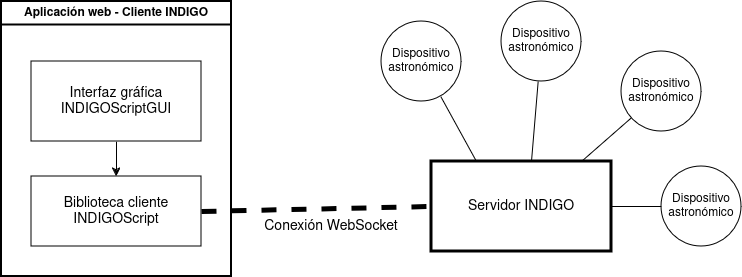
\includegraphics[scale=0.35]{img/arquitectura-client-server.png}
	\caption{Diagrama de arquitectura, se puede apreciar fácilmente la estructura cliente-servidor.}
\end{figure}

La biblioteca de INDIGO nos proporciona una implementación del servidor ya lista para su despliegue a través de la herramienta de línea de comando INDIGO Server. Este servidor es altamente extensible y soporta una gran cantidad de drivers, lo que permitirá centralizar el control de múltiples dispositivos astronómicos distribuidos de manera simultánea. Este servidor será un componente clave alrededor del cual diseñaremos nuestra aplicación. 

El servidor INDIGO hace uso de sus drivers y agentes para interpretar los parámetros de cada dispositivo astronómico y traducirlos en Propiedades, vectores de uno o más variables con nombre a través de las cuales se pueden controlar los parámetros del dispositivo.

INDIGO soporta 5 tipos de Propiedades:
\begin{itemize}
	\item Text: para el manejo de cadenas de texto.
	\item Number: para el control de valores numéricos.
	\item Switch: para valores binarios o de conmutacion.
	\item Light: para representar estados y alertas.
	\item BLOB: para manejar objetos binarios grandes, como imágenes o archivos de datos.
\end{itemize}

Originalmente, INDIGO transmite estas Propiedades a través de mensajes XML, pero también ofrece la posibilidad de usar un protocolo basado en JSON, lo cual nos será mucho más práctico para nuestra aplicación web. Se hará uso de WebSockets para la transmisión de estas Propiedades entre nuestro cliente web y el servidor de INDIGO.


\subsubsection{Arquitectura del cliente}

A continuación, se presenta la estructura de la aplicación web cliente:

%IMAGEN ESQUEMA ARQUITECTURA CLIENTE- Cliente JavaScript
\begin{figure}[h]
	\centering
	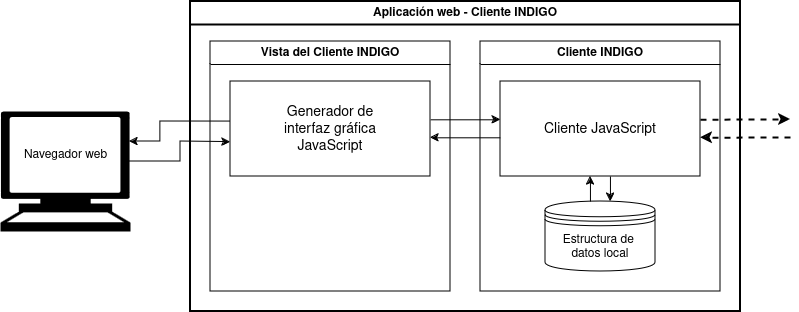
\includegraphics[scale=0.45]{img/arquitectura-appcliente.png}
	\caption{Estructura de la aplicación web cliente.}
\end{figure}

Este diseño de estructura se basa parcialmente en el patrón de diseño Modelo-Vista-Controlador (MVC).

En primer lugar, se plantea una capa primaria, el Cliente INDIGO. Esta capa estará compuesta por una clase en JavaScript que actuará como el Controlador de la aplicación. Este controlador será responsable de gestionar e interpretar los mensajes recibidos del servidor INDIGO, y coordinar la comunicación entre la interfaz de usuario y la estructura de datos. La estructura de datos en esta capa actuará como el Modelo, almacenando y gestionando de manera local los datos de las Propiedades.

En segundo lugar, se plantea una capa adicional, la Vista del cliente INDIGO, que asumirá el rol de Vista en el patrón MVC. Esta capa consistirá una clase en JavaScript cuya principal funcionalidad será la de inyectar elementos del DOM en el navegador, los cuales actuarán como interfaz gráfica de la aplicación, y permitiran una visualización de los datos en tiempo real.

Adicionalmente, se ha implementado el patrón Observador para gestionar el flujo de información entre la Interfaz Gráfica y el Cliente INDIGO. Este patrón permite que el Cliente notifique de manera automática a la Interfaz Gráfica según se reciban cambios en el Servidor, garantizando una interacción fluida entre los elementos de la aplicación.

\subsection{Implementación}

En estas fases iniciales, el enfoque principal ha sido el diseño preliminal de la aplicación, por lo que aún no se ha llevado a cabo ninguna implementación concreta. Se ha realizado una exhaustiva preparación de todas las herramientas que se utilizarán a lo largo del proyecto. Esto incluye la instalación de las bibliotecas INDIGO y de las herramientas gráficas (GUI) que estas ofrecen.

Asimismo, se ha creado un proyecto en TypeScript que servirá como base para todo el código que se desarrollará en el futuro. Se ha configurado el entorno de desarrollo integrado (IDE) Visual Studio Code para permitir la compilación automática de TypeScript a JavaScript, optimizando así el flujo de trabajo. Además, se ha incorporado la herramienta de empaquetado Rollup al proyecto, realizándose una serie de pruebas para garantizar su correcto funcionamiento.

Por último, se ha inicializado un repositorio en GitHub, que actualmente es privado, para gestionar el control de versiones del proyecto. Este repositorio será el espacio donde se alojará y se documentará todo el código fuente a medida que avance el desarrollo, asegurando así un seguimiento riguroso de las versiones y cambios realizados.


En estas fases iniciales, el enfoque principal ha sido el diseño preliminal de la aplicación, y por tanto aún no se ha llevado a cabo ninguna implementación de código destinado al proyecto. En su lugar, se han preparado y puesto a punto todas las herramientas que serán utilizadas a lo largo del proyecto. Esto incluye la instalación de la biblioteca INDIGO, el servidor INDIGO y de las herramientas gráficas que ofrece.

Se ha creado un proyecto en TypeScript que servirá como base para todo el código que se desarrollará en el futuro, y se ha configurado Visual Studio Code para permitir la compilación automática de TypeScript a JavaScript, para facilitar el desarrollo y hacerlo más cómodo. Además, se ha incorporado la herramienta de empaquetado Rollup al proyecto, y se han realizado una serie de pruebas para asegurar su correcto funcionamiento.

Por último se ha inicializado el repositorio en GitHub, actualmente privado, para gestionar el control de versiones del proyecto. En este repositorio se irá subiendo todo el código, además de la documentación, a medida que avance el proyecto.

\subsection{Pruebas}

Se han realizado las pruebas pertinentes para asegurar el correcto funcionamiento de las herramientas recién instaladas. 

\newpage

\section{Fase 5 - Sprint 1}

\subsection{Análisis}

Las historias introducidas en el Product Backlog de este sprint son las siguientes:

\begin{itemize}[leftmargin=10mm]
	\item \textbf{INDIGO.1.1  }Como desarrollador, quiero establecer una conexión con el servidor INDIGO haciendo uso del protocolo WebSocket
	
	\textbf{Prioridad:} Muy Alta
	\item \textbf{INDIGO.1.3  }Como desarrollador, quiero recibir mensajes del servidor en tiempo real a través de la conexión.
	
	\textbf{Prioridad:} Muy Alta
	\item \textbf{INDIGO.1.2  }Como desarrollador, quiero enviar mensajes formato JSON al servidor a través de la conexión WS.
	
	\textbf{Prioridad:} Muy Alta

	\item \textbf{INDIGO.1.5  }Como desarrollador, quiero que se almacenen en una estructura de datos las Propiedades que se reciban a través de mensajes y que no hayan sido almacenadas previamente.
	
	\textbf{Prioridad:} Alta
	\item \textbf{INDIGO.1.8  }Como desarrollador, quiero solicitar información sobre una o varias Propiedades específicas asociadas a un servidor.
	
	\textbf{Prioridad:} Alta

	\item \textbf{INDIGO.1.9 }Como desarrollador, quiero solicitar la información de todas las Propiedades asociadas a un servidor INDI.
	
	\textbf{Prioridad:} Media

\end{itemize}

Durante esta primera iteración, el objetivo principal es la inicialización de la clase en JavaScript que funcionará como cliente INDIGO. Las historias de usuario que componen el Product Backlog, si bien fundamentales para sentar las bases del cliente, no requieren un código excesivamente complejo. La mayor dificultad radicará en la familiarización con el sistema de mensajes del protocolo INDIGO y su correcta implementación en JavaScript/TypeScript.

\newpage

\subsection{Diseño}

Se ha diseñado el siguiente esquema de clase para planificar la clase del cliente y la estructura de datos de la que se valdrá:

%IMAGEN ESQUEMA ARQUITECTURA CLIENTE- Cliente JavaScript
\begin{figure}[h]
	\centering
	\hspace*{-2cm}   
	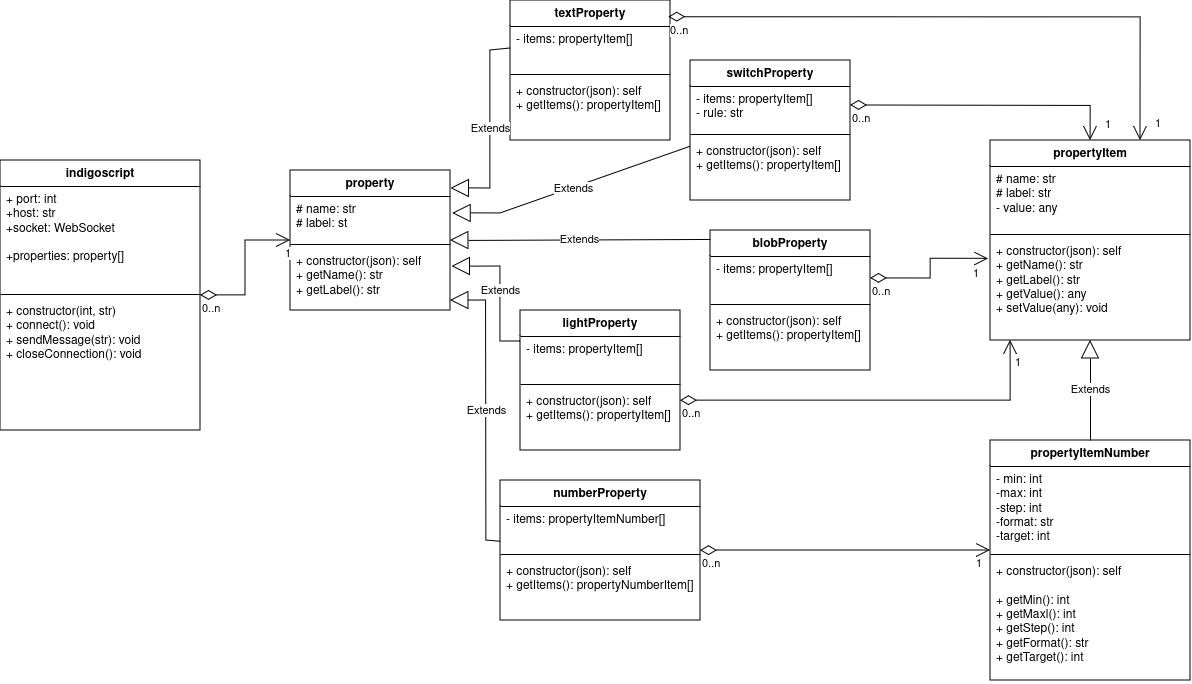
\includegraphics[scale=0.35]{img/diseño-sprint1.png}
	\caption{Esquema de clase diseñado para el sprint 1.}
\end{figure}

\subsection{Implementación}

Se implementan las historias de usuario de la siguiente manera:

\begin{itemize}[leftmargin=10mm]
	\item \textbf{INDIGO.1.1  Como desarrollador, quiero establecer una conexión con el servidor INDIGO haciendo uso del protocolo WebSocket.}\\
	\textbf{INDIGO.1.3  Como desarrollador, quiero recibir mensajes del servidor en tiempo real a través de la conexión.}
	
	Se han declarado variables de clase para almacenar la dirección del host y el puerto al que conectarse, y se ha creado una función 'connect()'. Esta función genera un objeto WebSocket haciendo uso de los datos almacenados para abrir una conexión con el servidor, y establece una serie de \textit{Event Listeners} que manejarán todo mensaje que llegue desde esta conexion. 

	\item \textbf{INDIGO.1.2  Como desarrollador, quiero enviar mensajes formato JSON al servidor a través de la conexión WS.}
	
	Aprovechando la conexión WebSocket creada, se añade una función 'send(message)' que permite el envió de mensajes a través del socket si este está definido. El envío es asíncrono, y la clase podrá seguir funcionando sin tener que interrumpir su ejecución en espera de una respuesta. En caso de recibir una, será captada por los 'Event Listeners' establecidos.

	\item \textbf{INDIGO.1.8  Como desarrollador, quiero solicitar información sobre una o varias Propiedades específicas asociadas a un servidor.}\\
	\textbf{INDIGO.1.9 Como desarrollador, quiero solicitar la información de todas las Propiedades asociadas a un servidor INDI.}
	
	Haciendo uso de las funciones de conexión con WebSocket recién declaradas, se añade la función 'sendGetPropertiesMessage(protocolVersion, deviceName? string, propertyName?: string)'. Esta función toma como parámetros opcionales el nombre de una propiedad específica y el del dispositivo al que pertenece, y construye y envia un mensaje 'getProperties' para solicitar las propiedades según estos parámetros. Esto nos permite solicitar todas las Propiedades del Servidor, las asociadas a un Dispositivo específico, o los datos concretos de una Propiedad en particular.

	\item \textbf{INDIGO.1.5  Como desarrollador, quiero que se almacenen en una estructura de datos las Propiedades que se reciban a través de mensajes y que no hayan sido almacenadas previamente.}
	
	Para el almacenamiento  de los datos correspondientes a los diferentes tipos de propiedades que se pueden recibir a través de los mensajes, se ha diseñado una estructura de datos basada en el principio de herencia de clases en una estructura basada en programación orientada a objetos.

Se ha implementado una clase genérica denominada 'Property()', con los datos principales de una propiedad como variables. A partir de esta clase genérica, se han derivado cinco clases especializadas: 'TextProperty()', 'NumberProperty()', 'SwitchProperty()', 'LightProperty()', y 'BlobProperty()', cada una correspondiente a un tipo específico de propiedad en el sistema INDIGO. Esto nos permite definir parámetros y funciones específicas para cada tipo de propiedad, eliminando redundancias en el código.

Adicionalmente, se ha creado la clase 'PropertyItem()', encargada de almacenar el nombre y valor de un ítem dentro de una propiedad. Esta clase también se extiende en la subclase 'PropertyItemNumber()', utilizada específicamente en las propiedades del tipo 'NumberProperty()' y que permite registrar los valores adicionales de este tipo de ítems.

Todas las clases definidas en esta estructura poseen un constructor que permite su creación a partir de un objeto en formato JSON. Con esta estructura declarada, en cuanto se reciba un mensaje del servidor con nuevas propiedades no tenemos más que invocar el constructor correspondiente y almacenarlo en la variable de clase 'indigoPorperties[]', que actuará como contenedor para todas las propiedades gestionadas por el cliente.

\end{itemize}

\subsection{Pruebas}

Para verificar el correcto envío y recepción de mensajes INDIGO desde JavaScript, se ha desarrollado una página HTML de prueba que permitirá crear una instancia del cliente con la que interactuar con el servidor. En esta página se han añadido una serie de botones que facilitan la prueba de las solicitudes getProperties mediante la función sendGetPropertiesMessages(). Además, se ha evaluado el almacenamiento de los datos recibidos en la estructura de datos recién implementada.

Después de realizar diversas pruebas, se ha confirmado que la conexión mediante WebSocket se establece sin inconvenientes y que el cliente es capaz de enviar y recibir mensajes con el servidor de manera efectiva.

\newpage

\section{Fase 6 - Sprint 2}

\subsection{Análisis}

Las historias introducidas en el Product Backlog de este sprint son las siguientes:

\begin{itemize}[leftmargin=10mm]
	\item \textbf{INDIGO.1.10 }Como desarrollador, quiero realizar cambios sobre las Propiedades almacenadas en la estructura de datos y enviar esos cambios a través de mensajes al servidor.
	
	\textbf{Prioridad:} Alta
	\item \textbf{INDIGO.1.4 }Como desarrollador, quiero que los mensajes recibidos sean procesados correctamente en función del tipo de respuesta (almacenar cambios en las Propiedades, procesar mensajes de error, notificaciones de conexión/desconexión...).
	
	\textbf{Prioridad:} Alta
	\item \textbf{INDIGO.1.6 }Como desarrollador, quiero que se actualicen automáticamente la estructura de datos de las Propiedades almacenadas al recibir mensajes con Propiedades almacenadas previamente.
	
	\textbf{Prioridad:} Alta
	\item \textbf{INDIGO.1.7 }Como desarrollador quiero que se verifiquen que los datos de las Propiedades almacenadas en la estructura de datos sean correctos y estén dentro de los rangos especificados, y que se detecten errores si se producen.
	
	\textbf{Prioridad:} Media
	\item \textbf{INDIGO.1.11 }Como desarrollador, quiero que las solicitudes de lectura o escritura de Propiedades se limiten/restrinjan en función de sus permisos (Read-only, Write-only, Read-write)
	
	\textbf{Prioridad:} Baja
	\item \textbf{INDIGO.1.12 }Como desarrollador, quiero que el State de una Propiedad (Idle, OK, Busy, Alert) se modifique automáticamente dentro de la estructura de datos al State correspondiente tras realizar modificaciones sobre dicha propiedad.
	
	\textbf{Prioridad:} Baja
\end{itemize}

En este segunda iteración, se terminarán de establecer las funcionalidades de nuestro cliente, haciendo un especial énfasis en la validación de datos. Al final de esta iteración dispondremos de un cliente web totalmente funcional y listo para ser usado en otras aplicaciones.


\subsection{Diseño}

Se ha diseñado el siguiente esquema de clase para planificar las funcionalidades implementadas en el cliente y las modificaciones realizada sobre la estructura de datos:

%IMAGEN ESQUEMA ARQUITECTURA CLIENTE- Cliente JavaScript
\begin{figure}[h]
	\centering
	\hspace*{-7cm}   
	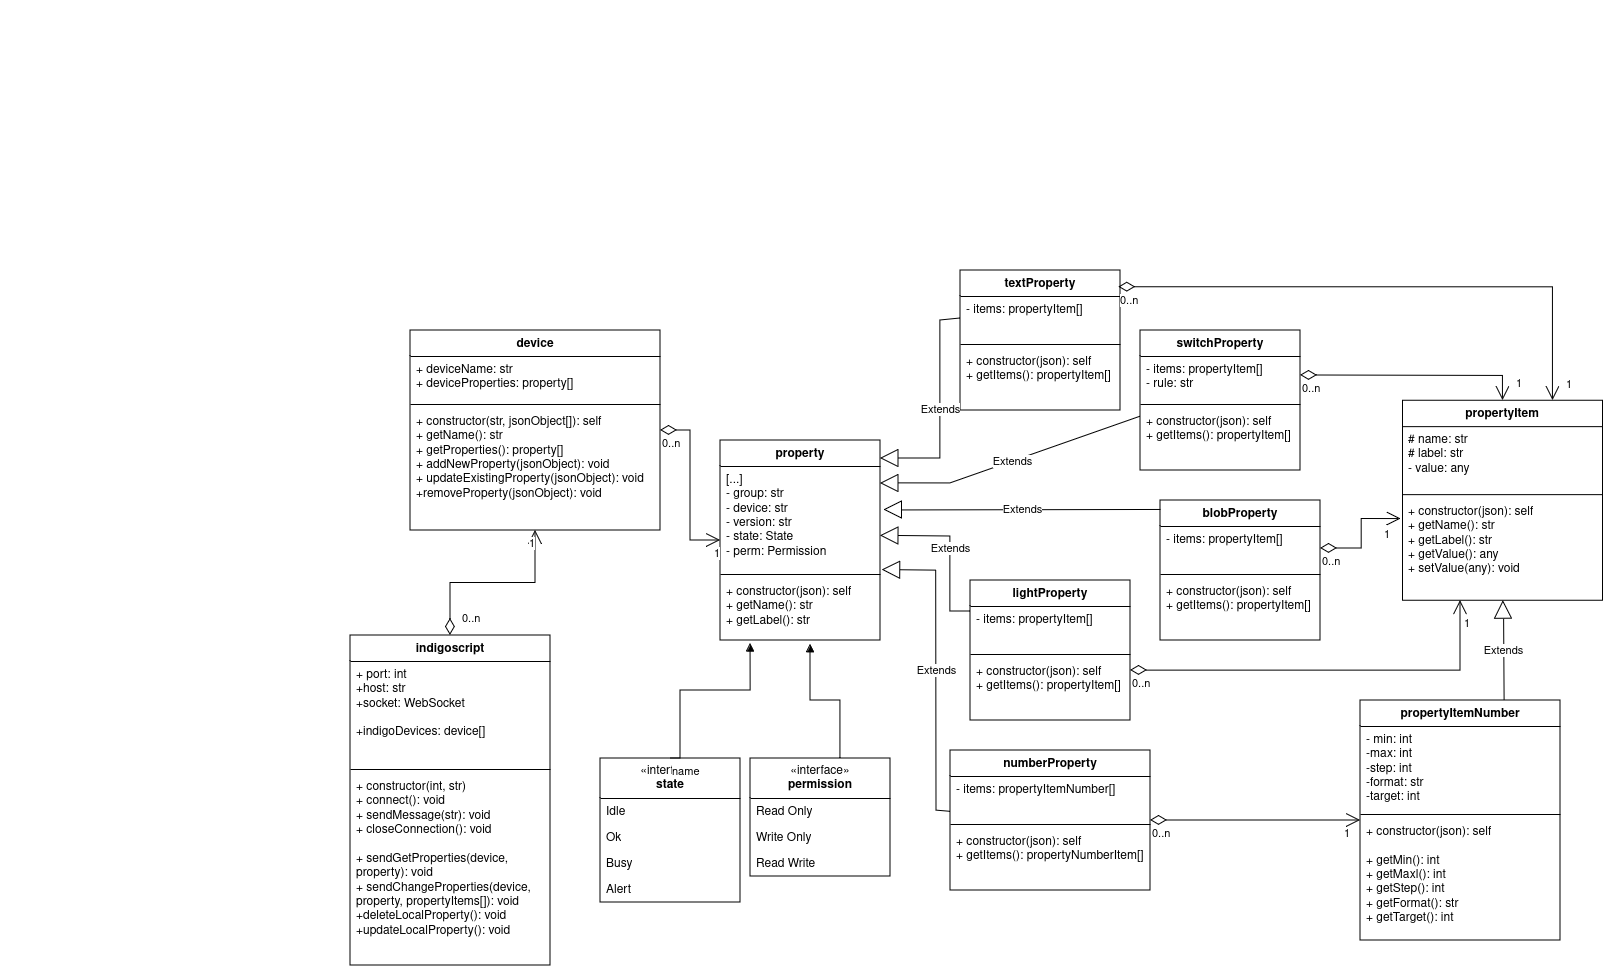
\includegraphics[scale=0.40]{img/diseño-sprint2.png}
	\caption{Esquema de clase diseñado para el sprint 2.}
\end{figure}


\subsection{Implementación}

\begin{itemize}[leftmargin=10mm]
	\item \textbf{INDIGO.1.10 Como desarrollador, quiero realizar cambios sobre las Propiedades almacenadas en la estructura de datos y enviar esos cambios a través de mensajes al servidor.}\\
	\textbf{INDIGO.1.12 Como desarrollador, quiero que el State de una Propiedad (Idle, OK, Busy, Alert) se modifique automáticamente dentro de la estructura de datos al State correspondiente tras realizar modificaciones sobre dicha propiedad.}
	Tomando como base la estructura de la función sendGetPropertiesMessages() desarrollada en el anterior sprint, se ha declarado la funcion sendChangePropertyMessage(), la cual toma como parámetros el nombre del dispositivo, el de la propiedad y uno o varios items cuyo valor modificar, organizados en un vector de Pares. La función redactará un mensaje JSON con los datos introducidos a través del Socket al servidor INDIGO.
	
	En caso de que el servidor acepte, implementará los datos recibidos en sus Propiedades y responderá al cliente con un mensaje 'getProperties' con los nuevos, y en caso de que no considere válidos estos cambios, enviará el mismo mensaje, reafirmando los datos no alterados al cliente. En ambos casos, el cliente recibirá una respuesta y actualizará su base local según el resultado, sin necesidad de realizar modificaciones directas sobre los datos de la estructura.
	
	\item \textbf{INDIGO.1.4 Como desarrollador, quiero que los mensajes recibidos sean procesados correctamente en función del tipo de respuesta (almacenar cambios en las Propiedades, procesar mensajes de error, notificaciones de conexión/desconexión...).}
	En el anterior sprint, todos los mensajes recibidos del Servidor eran tratados como un envío de propiedades, lo que podía dar lugar a errores en caso de recibir cualquier otro tipo de mensaje, como 'deleteProperty'. Se ha modificado la funcion 'connect()' para que se consulte la cabecera de los mensajes cada vez que se reciba uno, actuando según lo requiera el mensaje.
	
	\item \textbf{INDIGO.1.6 Como desarrollador, quiero que se actualicen automáticamente la estructura de datos de las Propiedades almacenadas al recibir mensajes con Propiedades almacenadas previamente.}
	
	En la anterior iteración cada vez que se recibía un mensaje con propiedades se creaba un objeto de la clase Property y sus derivadas, sin tneer en cuenta si ese objeto ya estaba registrado previamente. Para evitar la redundancia de datos se ha actualizado la función 'connect()' para que compruebe si una Propiedad ya está registrada antes de añadirla a la base local. En caso afirmativo, simplemente actualizará los valores de sus items en vez de crear una nueva.
\end{itemize}


Además, aparte de las historias de usuario implementadas, se han realizado cambios sobre la estructura de datos para representar de forma más precisa los dispositivos conectados al servidor. Se ha implementado una nueva clase 'Device()', que representará a un dispositivo y todas sus propiedades. La clase cliente tendrá acceso a un listado de dispositivos 'indigoDevices[]' en vez de acceder a un listado desorganizado de todas las propiedades. También se ha modificado la clase genérica 'property()' para incluir el resto de variables que definen a cada propiedad.


\subsection{Pruebas}


